\documentclass[12pt]{article}
\usepackage{placeins}
\usepackage{sbc-template}
\usepackage{float}
\usepackage{graphicx,url}
\usepackage{listings}
\usepackage[brazil]{babel}   
%\usepackage[latin1]{inputenc}  
\usepackage[utf8]{inputenc} 
\usepackage{color}
\definecolor{dkgreen}{rgb}{0,0.6,0}
\definecolor{gray}{rgb}{0.5,0.5,0.5}
\definecolor{mauve}{rgb}{0.58,0,0.82}
 
% UTF-8 encoding is recommended by ShareLaTex
\usepackage{}
\sloppy
\lstset{
  language=Python,                
  basicstyle=\footnotesize,           
  numbers=left,                   
  numberstyle=\tiny\color{gray},  
  stepnumber=2,                             
  numbersep=5pt,                  
  backgroundcolor=\color{white},    
  showspaces=false,               
  showstringspaces=false,         
  showtabs=false,                 
  frame=single,                   
  rulecolor=\color{black},        
  tabsize=2,                      
  captionpos=b,                   
  breaklines=true,                
  breakatwhitespace=false,        
  title=\lstname,                               
  keywordstyle=\color{blue},          
  commentstyle=\color{dkgreen},       
  stringstyle=\color{mauve}, }

\title{Segundo Projeto de Comunicações Móveis}

\author{Vítor Gabriel Lemos Lopes}


\address{Departamento de Engenharia de Comunicações-UFRN
}

\begin{document} 

\maketitle

     
\begin{resumo} 
  Este Trabalho foi feito com intuito de aprendizado sobre comunicações digitais, e sobre os tipos de canais mais utilizados nas comunicações, e como se comportam,a probabilidade de erro de cada um dos canais. Para isso foi utilizado a linguagem de programação em Python para a modelagem dos canais e a probabilidade de erro de cada canal, com isso foram feitos gráficos para comparação do simulado com a probabilidade de erro teórica.
\end{resumo}
\section{Introdução}
 Como sabemos a transmissão sem fio dois principais tipos de atenuação, Desvanecimentos em larga escala e o desvanecimento em pequena escala. Este projeto tem como objetivo estudar o desvanecimento em pequena escala em um sistema de comunicação digital sem fio. \\
 Na comunicação digital é estudado a quantidade de erros de bits para poder fazer uma transmissão confiável, neste trabalho vamos estudar os canais mais comuns utilizados que são: Canal AWGN(\textit{Additive White Gaussian Noise} e o canal de \textit{Rayleigh}, vamos fazer uma simulação com cada canal com o efeito de atenuação feita por esses canais ruidosos entre a modulação e demodulação e utilizar o valor da probabilidade de erro de bit teórica para comparar com o simulado.
 

\section{Experimento 1} \label{sec:firstpage}
Para o primeiro Experimento foi pedido que fosse feita duas simulações, uma da constelação de bits com a adição do ruído AWGN e um gráfico comparando a probabilidade de erro de bits teórica com a simulada. Para isto foi criado um sinal antipodal sem formatação de pulso, e o ruido AWGN foi feito uma variável aleatória gaussiana com média 0 e variância $N0/2$, que é dado nos livros de referência, o qual $N0$ é:
\begin{equation}
    N0= Eb * 10^{-SNR_{dB}/10}
\end{equation}
Os quais:
\begin{itemize}
    \item \textbf{N0}:Densidade espectral do ruído.
    \item \textbf{Eb}: Energia de bit dado no problema.
    \item \textbf{SNR}: Relação sinal ruído em dB dado no problema.
\end{itemize}

\subsection{Constelação}
Para poder modelar o gráfico da constelação é necessário criar um sinal antipodal que foi criado com ajuda da biblioteca Numpy do Python e foi da seguinte forma:
\begin{lstlisting}
bit=np.random.randint(0,2,size=b)
sinal=np.where(bit==0,-1,bit)
\end{lstlisting}
Qual foi criado um vetor aleatório de 0 e 1, e depois modificado para onde tem o bit 0 ser colocado para -1, Para o sinal ser um BPSK. O tamanho do vetor foi definido a quantidade de bits que serão transmitidos, que no caso da questão são 100 bits.

\begin{figure}[h]
    \centering
    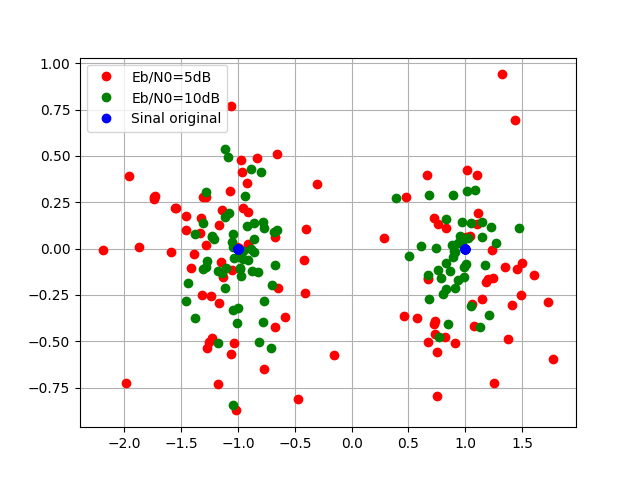
\includegraphics{constelacao.png}
    \caption{Constelação de bits}
    \label{fig:my_label}
\end{figure}
Com este gráfico podemos observar uma nuvem envolta do sinal original, isso é devido a adição do ruído AWGN, que como foi falado anteriormente é uma variável aleatória, só que o ruído possui componente real e imaginária, por isso vemos componentes em x e y.
E podemos ver também que quanto menor o $Eb/N0$(que é a nossa SNR da formula 1) mais espalhado são os bits que chegam no receptor, pela formula 1 podemos perceber que quanto maior a SNR, menor é a densidade espectral do ruído isso fazendo a variância do AWGN diminuir significadamente, como vimos que o ruído é a variável aleatória que depende da média e da variância,já que a média é zero, a variância quanto menor menos ele vai se afastar do ponto inicial.
\subsection{Probabilidade de erro de bits}
Para um canal AWGN a probabilidade de erro teórica dado nas referências é:
\begin{equation}
    Pe=Q\left(\sqrt{\frac{2Eb}{N0}}\right)  
    
\end{equation}
\textbf{Ou} \begin{equation}
    Pe=\frac{1}{2}erfc \left(\sqrt{\frac{Eb}{N0}}\right)
    \end{equation}
Agora para criação do sinal simulado fazemos os procedimentos descritos anteriormente, com algumas modificações, para definirmos os sinais errados, é pego o sinal recebido que é igual o sinal original(com -1 e 1) somado ao ruido AWGN, fazemos um limiar de decisão com esse código:
\begin{lstlisting}
resultbit=np.where(sinalrecpt>=0,1,-1)
\end{lstlisting}
Onde para todos os bits que chegam que são maiores que 0 são 1, e todos os menores que 0 são -1. Com isso fazemos a comparação e contamos quantos erros temos e dividimos pela quantidade de bits que foram transmitidos.
\begin{lstlisting}
bit_error=np.where(sinal!=resultbit,1,0)            
ber.append((sum(bit_error))/b)
\end{lstlisting}
Com essas informações podemos plotar os gráficos:
\begin{figure}[h!]
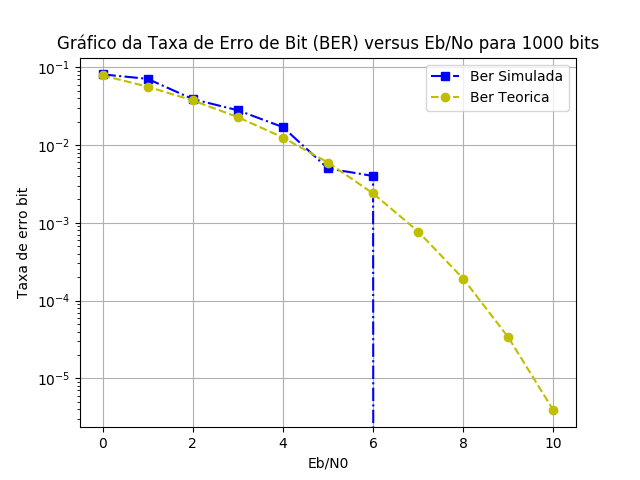
\includegraphics[width=0.98\textwidth]{bermil.png}
    \caption{Probabilidade de erro com mil bits}
    \label{fig:my_label}
\end{figure}
\FloatBarrier
\begin{figure}[h!]
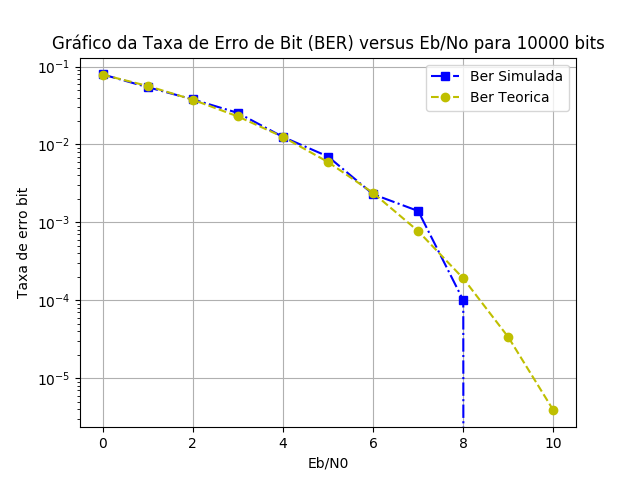
\includegraphics[width=0.75\textwidth]{ber10mil.png}
    \caption{Probabilidade de erro com 10 mil bits}
    \label{fig:my_label}
\end{figure}
\FloatBarrier

\begin{figure}[h!]
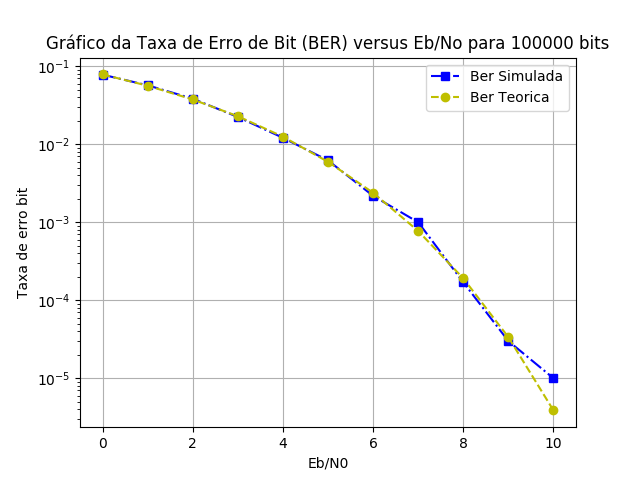
\includegraphics[width=0.75\textwidth]{ber100mil.png}
    \caption{Probabilidade de erro com 100 mil bits}
    \label{fig:my_label}
\end{figure}
\FloatBarrier
Podemos perceber que com aumento do Eb/N0 a probabilidade de erro de bits diminui, isso é devido a que os bits ficam menos espalhados e mais próximos  do sinal original assim acontecendo uma menor quantidade de erros de bits. Também é possível perceber nos gráficos que a quantidade de erro de cai pra zero em uma quantidade de bits menor, isso significa que não há bits suficientes para poder estimar a BER até os 10 dB de Eb/N0.
\section{Experimento 2}
Neste experimento foi pedido para estimar um canal com desvanecimento plano (AWGN+ Rayleigh fading) para isso vamos calcular a probabilidade de erro de bit, chamando SNR de $\gamma$, é dada pela formula:
\begin{equation}
    \int_{0}^{\infty} P^{AWGN}(\gamma )p(\gamma)d\gamma
\end{equation}
Para uma modulação BPSK a probabilidade do AWGN já foi dado na equação 2 e 3. e a distribuição da SNR em um canal com desvanecimento de Rayleigh é:
\begin{equation}
    p(\gamma)= \frac{1}{\gamma_{b}}e^{\frac{-\gamma}{\gamma_{b}}}
\end{equation}
Onde $\gamma _{b}$ é a SNR média, colocando de novo na equação:
\begin{equation}
    \int_{0}^{\infty} Q(\sqrt{2\gamma})\frac{1}{\gamma_{b}}e^{\frac{-\gamma}{\gamma_{b}}}d\gamma = \frac{1}{2}\left(1-\sqrt \frac{\gamma _{b}}{1 +\gamma _{b}}\right)
\end{equation}
Que foi usada para calcular a probabilidade teórica do canal plano. E para o canal simulado foi criada a variável h(t) dada pela formula que está nas referências:
\begin{equation}
    h(t)=\sqrt{\frac{X^{2}+Y^{2}}{2}}
\end{equation}
 X e Y são duas variáveis aleatórias gaussianas diferentes, com média zero e desvio padrão 1, fazendo o sinal recebido ser:
 \begin{equation}
     SinalRecpt=sinal*h(t)+AWGN
 \end{equation}
Sendo possível modelar o Gráfico:
\begin{figure}[h]
    \centering
    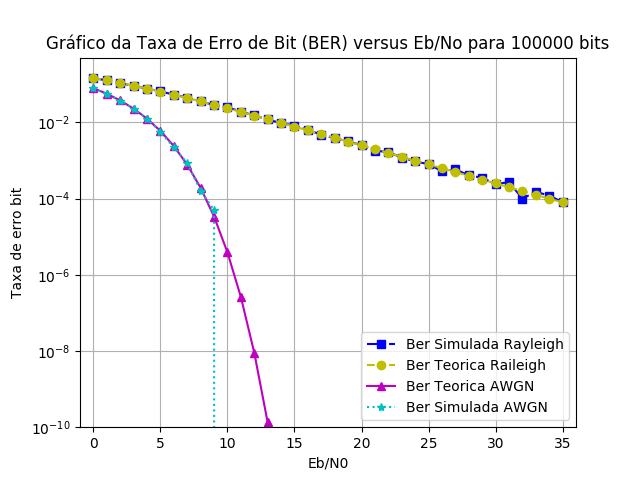
\includegraphics[width=0.7\textwidth]{ray.png}
    \caption{Comparação de canais}
    \label{fig:my_label}
\end{figure}
\FloatBarrier
Com isso é possível ver que em 35 dB de SNR chega a uma probabilidade de erro em $10^{-4}$ no canal de Rayleigh, já no AWGN atinge essa probabilidade em 8 dB, ou seja  canal de Rayleigh é um canal com um ruído muito maior que um canal AWGN e não é tão eficaz quanto o AWGN com o aumento da SNR.



\section{References}
\cite{comuni:18}
\cite{Haykin:01}
\cite{proakis:11}

\bibliographystyle{sbc}
\bibliography{sbc-template}
\end{document}
